\section{Resultados e discussão}

Para encontrar todos os resultados necessários para comprovar a teoria, a prática foi dividida em algumas etapas, sendo elas:


\begin{itemize}

    \item Aplicar uma senoide de 0.5 V de amplitude e 150 hz de frequência na entrada do circuito da figura \ref{ckt:1}
    e comparar as formas de onda obtidas no nó $V_o$ com os resultados teóricos;
    
    \item Aplicar a mesma senoide do experimento anterior no circuito da figura \ref{ckt:2} e comparar as formas de onda obtidas no nó $V_o$ e $V_{o1}$ com os resultados teóricos.
\end{itemize}

Antes dos circuitos serem montados, os diodos foram testados separadamente para garantir que não estejam funcionando na região de ruptura. Só assim foram montados os circuitos da figura \ref{ckt:1} e \ref{ckt:2}.

Ao obter as medições, para conferir se os resultados corroboram com a prática, foi adotado um erro de 5\% como uma boa figura de mérito para avaliar o desempenho dos circuitos. Caso contrário o circuito deveria ser revisado em busca de reduzir o ruído ou qualquer resistor com resistência fora da faixa de tolerância. 

No que confere a saída $V_o$ do circuito da figura \ref{ckt:1}, foram obtidas as formas de onda da figura \ref{fig1}.

\begin{figure}[H] 
\centering
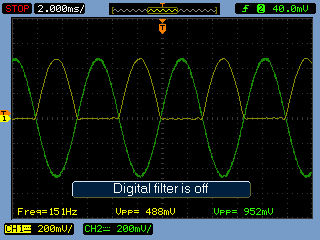
\includegraphics[width=7.5cm]{images/VO_1.png}
\caption{Comparação entre entrada (CH2) e saída (CH1) do retificador de meia onda.}
\label{fig1} 
\end{figure}

Observa-se que a relação teórica entre o valor de entrada e saída foi obedecida na prática, com um erro de apenas 2.4\%, visto que no semi-ciclo negativo da entrada esperava-se um valor de 500mV de amplitude para o sinal de saída, mas só obteve-se 488mV. 

Outro fato importante é que a frequência do sinal de saída permaneceu a mesma do sinal de entrada (150Hz), pois no semi-ciclo positivo da entrada, a saída permaneceu nula.

Na segunda parte foi conferida a saída $V_o$ do circuito da figura \ref{ckt:2}, obtendo-se as formas de onda da figura \ref{fig2}

\begin{figure}[H] 
\centering
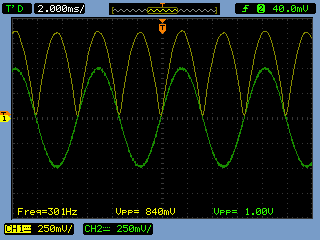
\includegraphics[width=7.5cm]{images/VO_2.png}
\caption{Comparação entre entrada (CH2) e saída (CH1) do retificador de onda completa.}
\label{fig2} 
\end{figure}

Observa-se que a relação teórica entre o valor de entrada e saída foi obedecida na prática, com um erro de apenas 4.76\%. Isso, pois a amplitude do sinal de saída é 840mV para um valor esperado de 882mV. 

Diferente do amplificador de meia onda, o amplificador de onda completa possui sinal na saída para ambos os ciclos (positivo e negativo) do sinal de entrada. Porém, a ele está associado um ganho de $1.68$, cujo valor teórico é $1.76$, permitindo que sua amplitude seja diferente da amplitude do sinal de entrada. 

Como a saída possui resposta não nula para ambos os ciclos do sinal de entrada, implica que a frequência do sinal na saída dobrou de valor.

Também foi conferida a forma de onda no nó de tensão $V_{o1}$ do circuito da figura \ref{ckt:2}, gerando a figura \ref{fig3}.

\begin{figure}[H] 
\centering
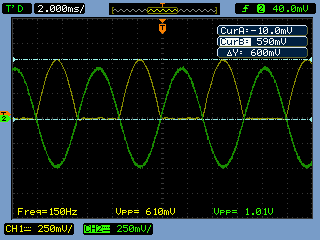
\includegraphics[width=7.5cm]{images/VO1.png}
\caption{Comparação entre entrada (CH2) e o ponto $V_{o1}$ (CH1) do retificador de onda completa.}
\label{fig3} 
\end{figure}

Observa-se que nessa parte do circuito, a forma de onda obtida é nada mais que o resultado de uma amplificação de meia onda, ou seja, a saída será a contribuição desse nó do catodo desse diodo com o nó do anodo do outro diodo. E o valor nesse ponto corrobora com seu valor teórico obtido anteriormente, possuindo um erro de apenas1\%. Isso, pois a amplitude do sinal no nó $V_{o1}$ é 590mV para um valor esperado de 588mV. 


Vale destacar que em ambos circuitos a amplitude do sinal de entrada foi menor do que a tensão de polarização usual de um diodo (0.7 V). Isso implica que em retificadores normais que não se valem do uso do conjunto AMPOP/diodo, esse sinal não teria amplitude suficiente para ser retificado, logo implicando em uma saída nula para o caso de um retificador de meia onda e onda completa com o uso de diodos. Porém no caso dos retificadores de precisão essas dificuldades foram superadas devido ao uso do "super-diodo".

\newpage